\section{Memory} \label{subsec:Memory}
The FPGA has internal memory to store settings for the ADCs, DACs and sample memory. It has a total of 16x24 bit internal memory that can be accessed by the MCU. This memory can easily be expanded by changing a single line of code if there was ever a need for it.

The code for the memory can be seen on listing \refq{lst:7_2_2_MemoryCode} and will be explained with the block diagram on figure \refq{fig:7_2_2_MemoryBlock}. To write to, or read from, memory is a two-step process. First the module requires an address and then it can either read from, or write to, from that address. An asynchronous reset is checked, if no reset is required, the state machine will at each rising clock of the MCU clock perform an action. At each rising edge of the clock, the system will check if the MSB of register 7 is set to a 1. If this is the case, it will set register 7 to x"0000". The MSB of register 7 is used to initiate a sample sequence, so the MCU can program in the MSB to a logic '1', this will then have the system take whatever amount of samples that has been requested. The next time the MCU communicates with the internal memory, register 7 will automatically be reset to 0, allowing for a new set of samples to be taken. Lines 37 to 50 shows how the internal registers are synchronously updated with the \SIQ{200}{\mega\hertz} master clock

\lstinputlisting[language=c ,style = c,firstnumber=1, linerange=67-116, caption={Code for the memory inside the FPGA}, label={lst:7_2_2_MemoryCode}]{Sections/7_SystemDesign/Code/internal_ram.vhd}

Lines 1-7 are type declarations of the RAM, which specifies it's size as 16x24 bit block RAM along with a state variable declaration used for the writing to the RAM. The memory is not a pure finite state machine as there are separate branches for the read and write modes. Everything inside the memory, whether they be reads or writes, happens at the rising edges of the CLK signal as indicated by line 14 and CLK the transitions marked on the block diagram on figure \refq{fig:7_2_2_MemoryBlock}. The memory can either be set to a read, or a write mode. If the memory is set to write mode it will enter a finite state machine at line 21 and will alternate between the two states shown on the right side of figure \refq{fig:7_2_2_MemoryBlock} for as long as RW = '0'. All writes to the memory starts with an address that will be saved to an Address variable on the rising edge of the CLK, afterwards the state machine will transition to the 'Save Data' state and a CLK to this save will save the data in the memory at the address. The state machine will cycle between these two states for as long as RW is asserted. 



\begin{figure}[H]
    \centering
    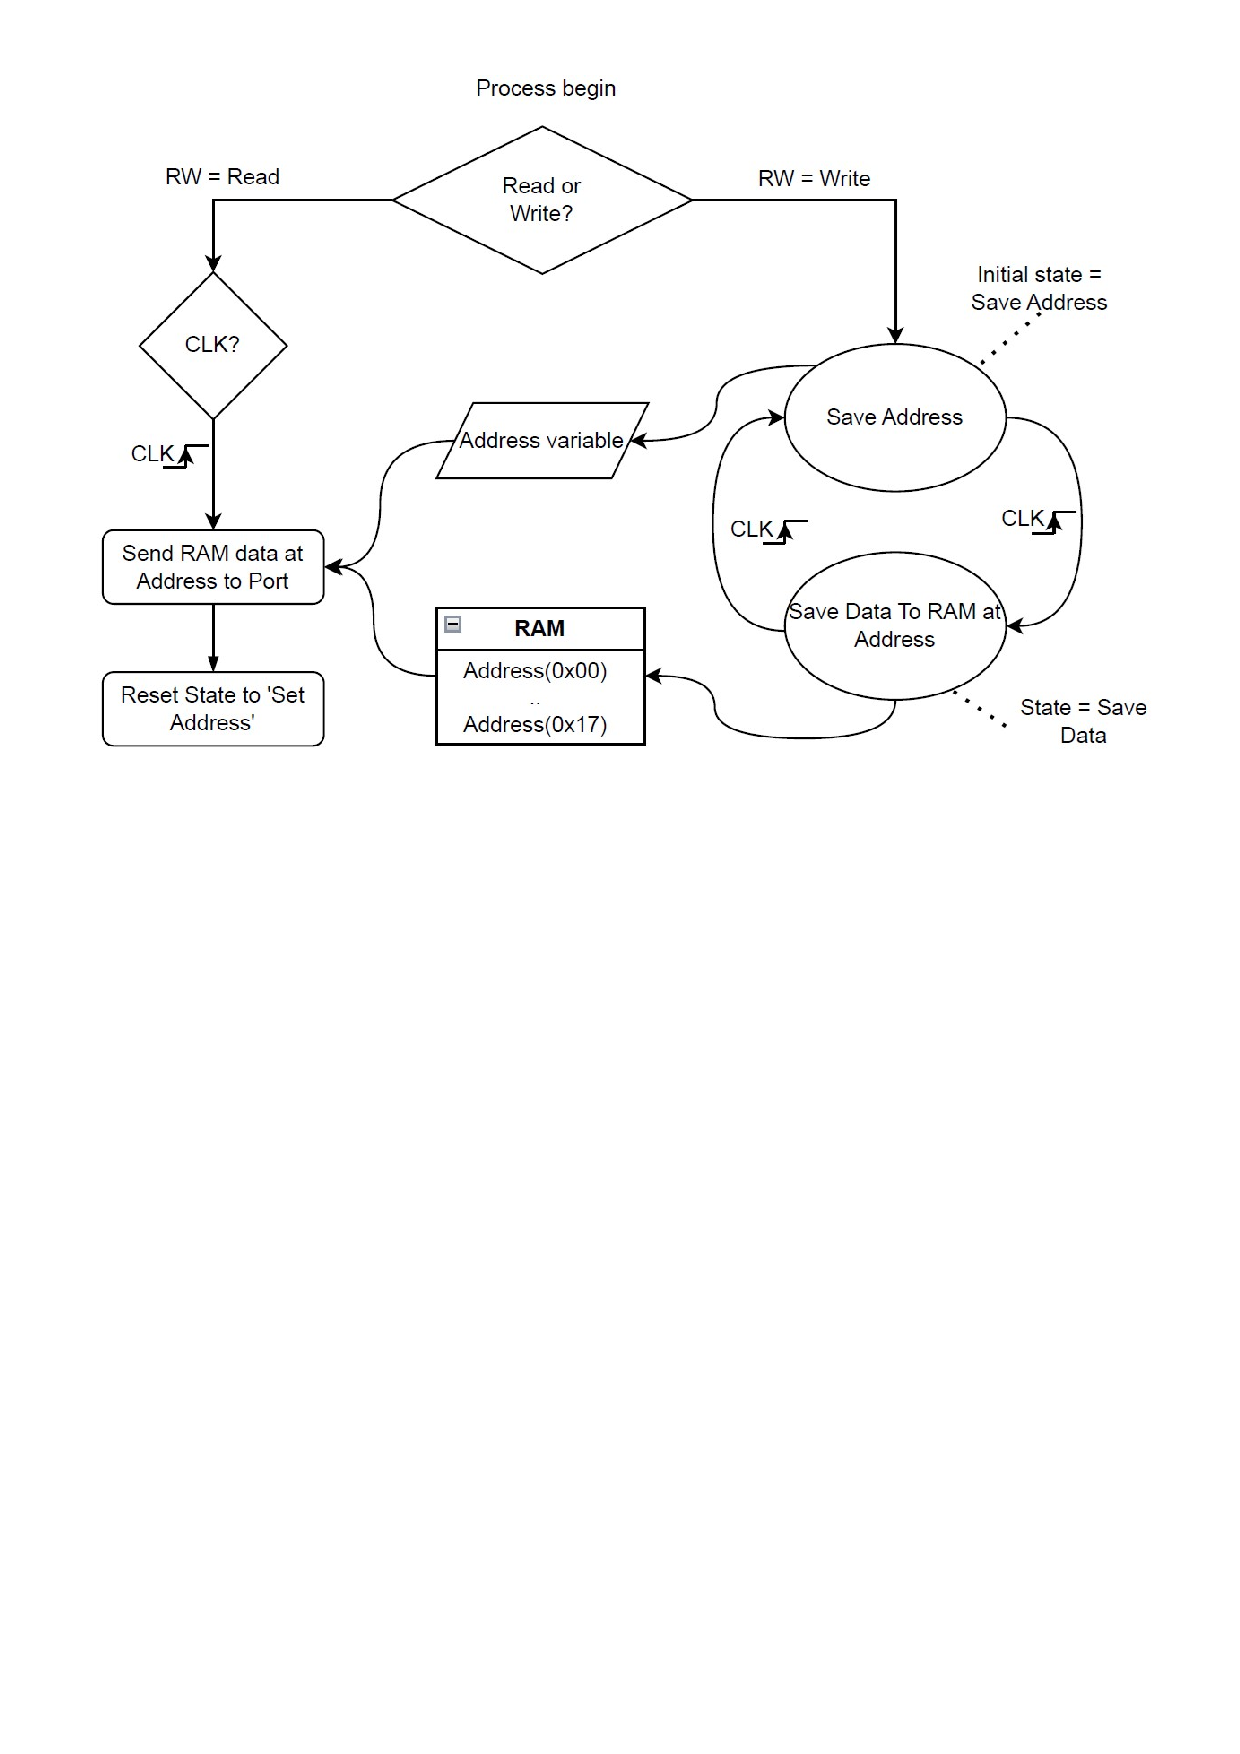
\includegraphics[clip, trim=0 450 0 0, width=1\textwidth]{Sections/7_SystemDesign/Figures/7_2_2_MemoryBlockDiagram.pdf}
    \caption{The module can either read a store value from memory(left), or it can store a value in memory. (right)}
    \label{fig:7_2_2_MemoryBlock}
\end{figure}

In order to read from the memory an address will have to be written to memory before changing to read mode, this means the finite state machine should be CLK'd through the first state before reading from memory. When the memory is in read mode it will enter the left branch of the block diagram on figure \refq{fig:7_2_2_MemoryBlock} and, at the first CLK, will send the data at the specified RAM address to the communication port (I/O tri-state buffers). When this is done it will reset the state machine to accept a new address.

\subsection*{Logic Reset}
The asynchronous reset in listing \refq{lst:7_2_2_MemoryCode} is controlled by another FSM. It has proven useful to have a way to reset the different modules to their default state, and as such the Logic Reset module has been designed. One reason for this is that when the STM32F446RE microcontroller boots it will toggle it's output pins, this includes toggling the CLK signal for the communication bus. This means the application software on the STM32F446RE can't know what state the memory state machine is in. In order to solve this there is an extra bit of logic that the MCU can use to reset the state machine to it's default value of 'state = Set Address' and this way the STM32 will have control over the process. This bit of code is shown in list \refq{lst:7_2_2_LogicReset}. 

\lstinputlisting[language=c ,style = c,firstnumber=1, linerange=59-95, caption={A piece of hardware the MCU can use to reset the memory modules state variable.}, label={lst:7_2_2_LogicReset}]{Sections/7_SystemDesign/Code/logic_reset.vhd}

The reset logic is implemented as a finite state machine that will, after a number of state transitions toggle the reset signal to create a pulse that will reset the memory. The state machine is shown on figure \refq{fig:7_2_2_ResetLogicFSM}. 

\begin{figure}[H]
    \centering
    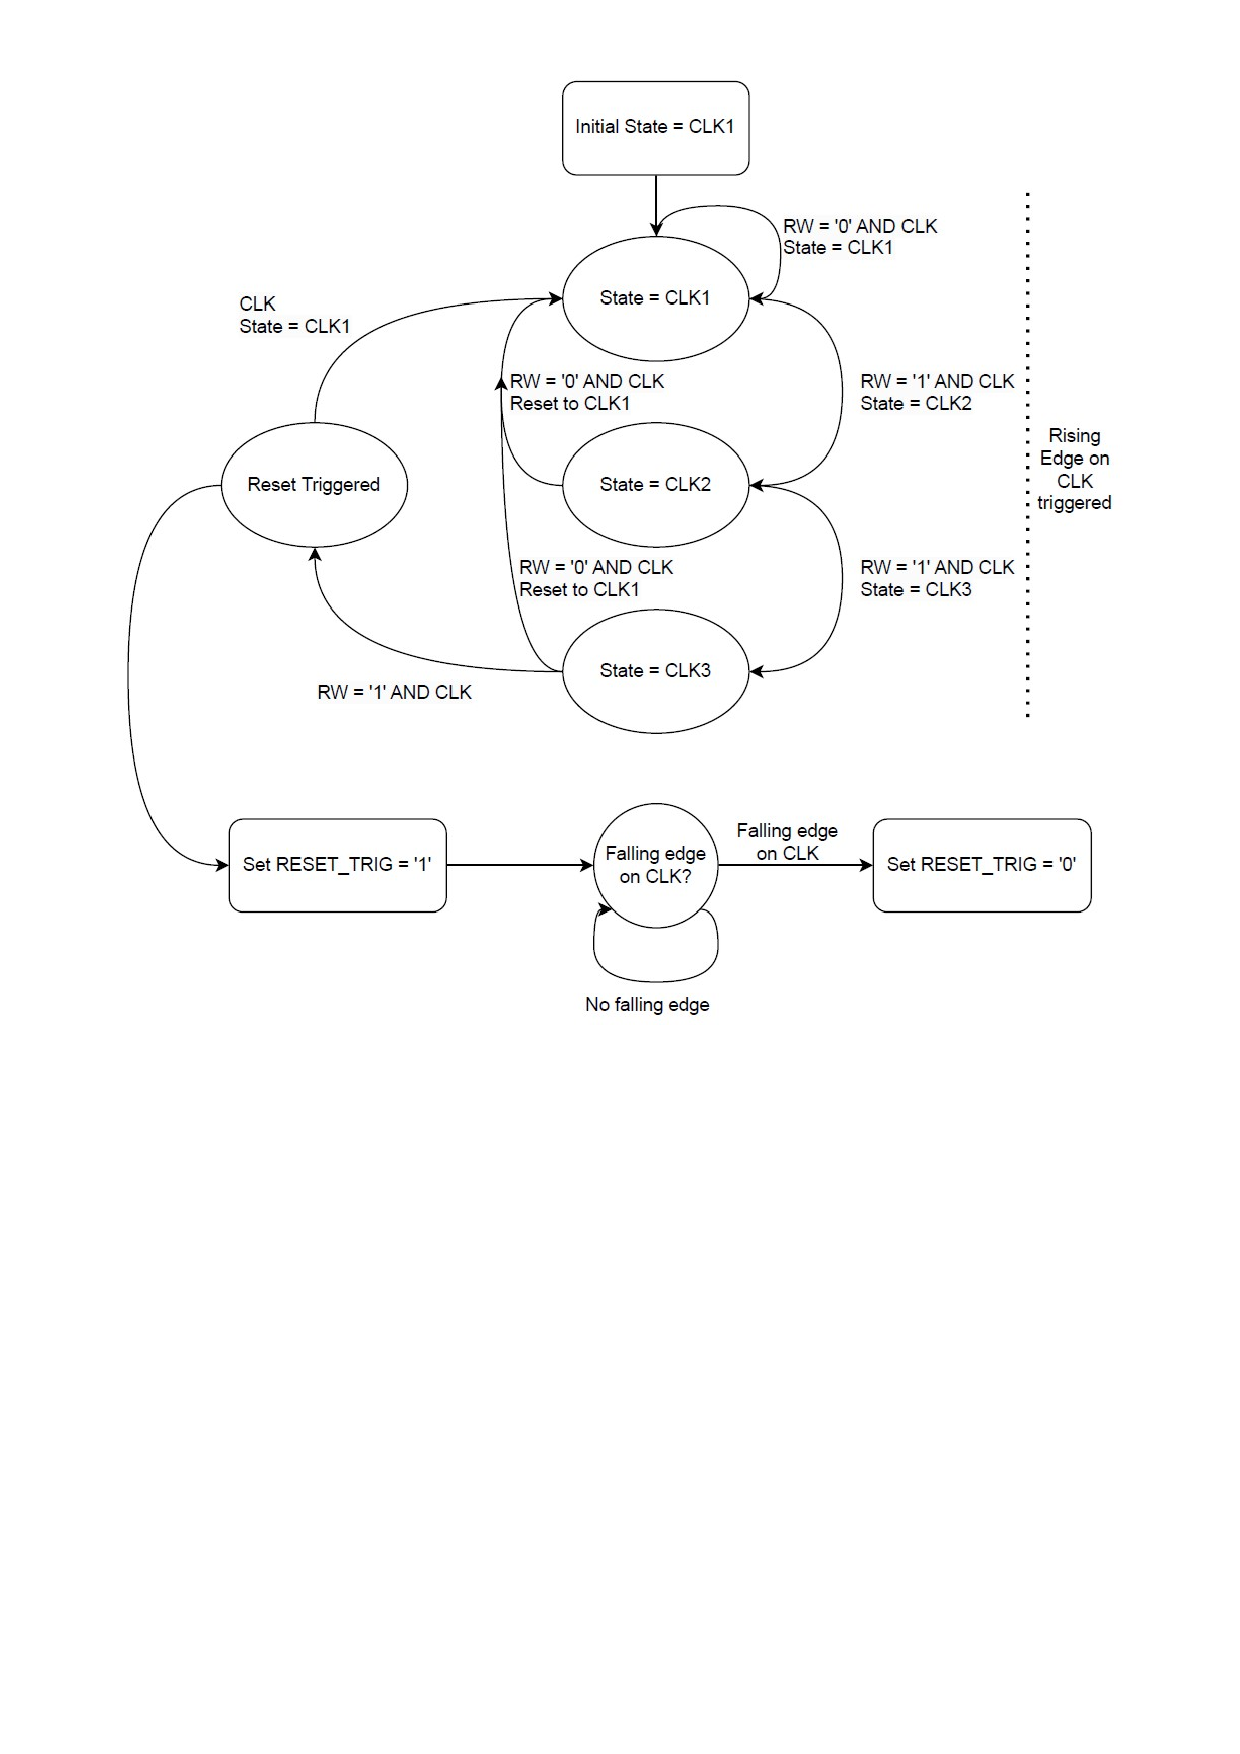
\includegraphics[clip, trim=0 0 0 0, width=1\textwidth]{Sections/7_SystemDesign/Figures/7_2_2_ResetLogicFSM.pdf}
    \caption{The reset logic implemented as a finite state machine. The state transitions all happen on a rising edge of the CLK signal as indicated on the right side of the figure. If RW = '1' while a rising edge on CLK happens, then the state machine will transition to the next state.}
    \label{fig:7_2_2_ResetLogicFSM}
\end{figure}

The microcontroller will have to follow a sequence of events in order to trigger a reset of the memorys state variable as shown in the code, and on figure \refq{fig:7_2_2_ResetLogicFSM}. If RW and IX are held at '1' for 3 consecutive rising edges of the CLK then it will trigger a reset on the 4th rising edge of the CLK. If the RW is released, so RW = '0', at any point during this sequence then the reset logic state machine will reset to it's default state. When the 'reset triggered' state is reached the reset signal will go to '1' and will self-reset at the falling edge of the 4th CLK pulse as shown in the top of figure \refq{fig:7_2_2_ResetLogicFSM}. This means the reset signal has the same pulsewidth as the clock signal.